Die Variable \verb+participant+ wird benutzt um für den Fall, dass die Wahl
von zwei Knoten gestartet wurde, einen Ausfall des Prozesses mit der höchsten
Prozessnummer (also dem zukünftigen Leader) kompensieren zu können.
Im Beispiel in Abbildung \ref{fig:9_1_start} starten 2 Knoten unabhängig voneinander
eine Wahl. Jeder Knoten reagiert entsprechend dem Algorithmus von Seite 11 im
Vorlesungsskript. Alle Knoten bis auf 6, die eine Nachricht verschickt haben,
haben \verb+participant+ auf \verb+true+ gesetzt. \\
Erhält nun der Knoten 5 die Nachricht \verb+<election, 4>+, also eine
Nachricht aus dem nicht von ihm gestarteten Wahlprozess, so ernennt er sich selbst
zum Leader und schickt dies als Nachricht an den folgenden Prozess (siehe
Abbildung \ref{fig:9_1_firstleader}). Alle Prozesse aktzeptieren zunächst 5 als
Leader. \\
Irgendwann erreicht auch die Wahlnachricht \verb+<election, 6>+ (als Teil
der ursprünglich von 5 initiierten Wahl) Knoten 5. Dann gibt 5 seinen Leaderstatus wieder ab
und 6 wird zum Leader gewählt (siehe Abbildung \ref{fig:9_1_final}).
Die Variable ist also nicht essentiell für den Algorithmus. Ohne
\verb+participant+ müsste man einen Ausfall erkennen (beispielsweise durch
einen Timeout) und eine neue Wahl veranlassen. \\
Mit \verb+participant+ hingegen wird auch bei Ausfall eines Prozesses ein Leader gewählt. Es dauert nur
länger bis tatsächlich der Prozess mit der höchsten Prozessnummer als Leader
gewählt ist.
\begin{figure}
  \begin{center}
    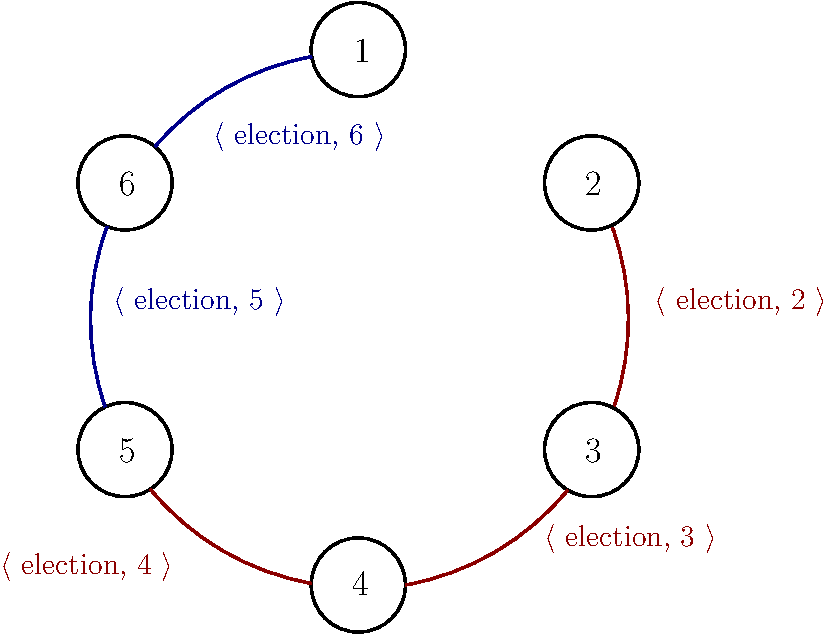
\includegraphics{pics/9_1_1.pdf}
  \end{center}
  \caption{Knoten 2 und 5 starten eine Wahl}
  \label{fig:9_1_start}
\end{figure}

\begin{figure}
  \begin{center}
    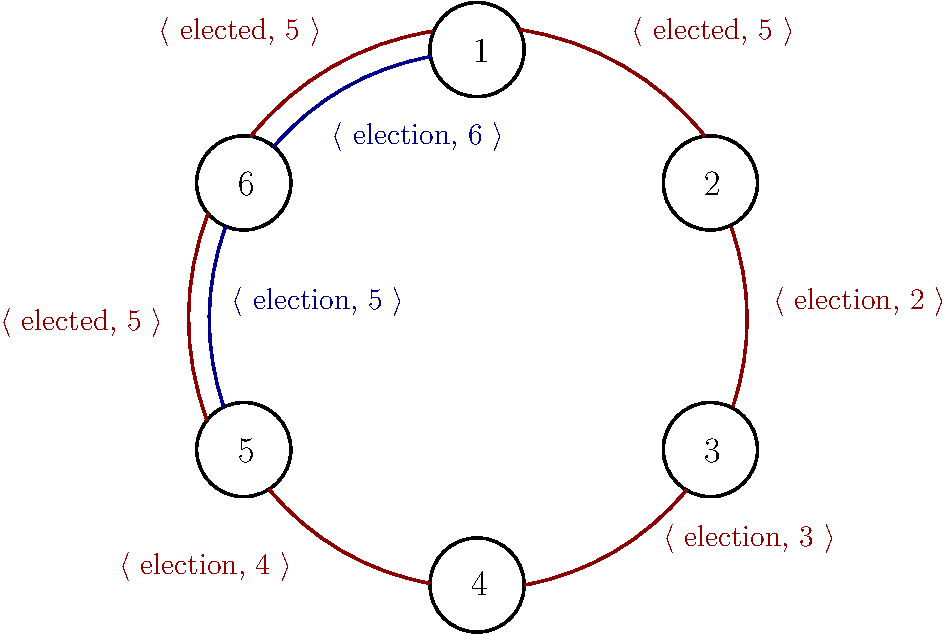
\includegraphics{pics/9_1_2.pdf}
  \end{center}
  \caption{Knoten 5 ernennt sich selbst zum Leader}
  \label{fig:9_1_firstleader}
\end{figure}

\begin{figure}
  \begin{center}
    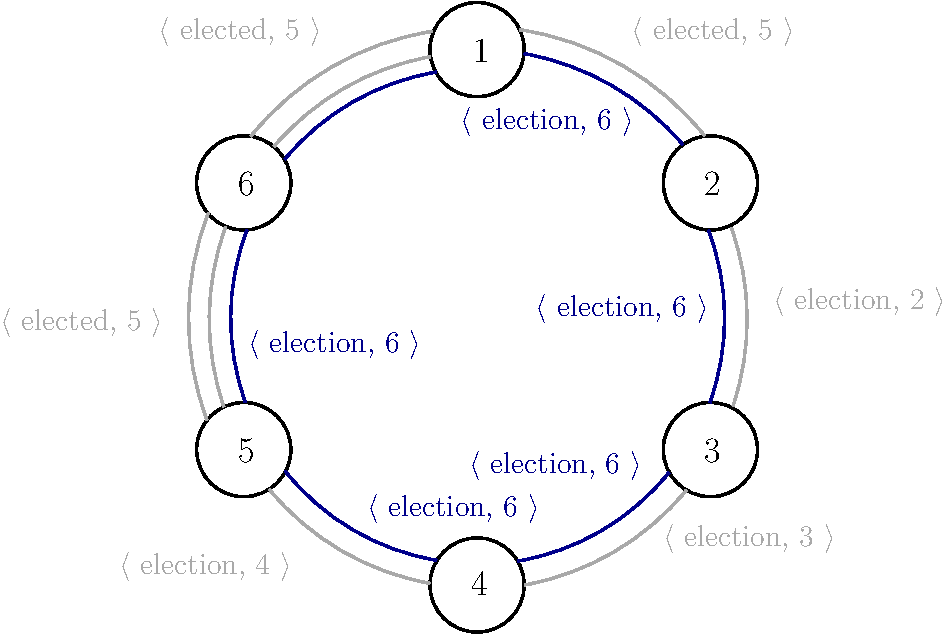
\includegraphics{pics/9_1_3.pdf}
  \end{center}
  \caption{Knoten 6 wird letztendlich zum Leader gewählt}
  \label{fig:9_1_final}
\end{figure}
